\section{Model Room Illuminance Calculation}
The algorithm was tested on a model room of dimension $\left(10 \times 5 \times 4\right)$~m. Any barriers or equipment were not considered. Pure diffuse reflections were considered with facets reflectance:
\begin{itemize}
	\item $\rho = 0.2$ for floor,
	\item $\rho = 0.5$ for walls,
	\item $\rho = 0.7$ for ceiling.
\end{itemize}
Each facet has the same dimension $\left(0.25 \times 0.25\right)$~m. $4$~reflections were evaluated for each solution. High count of reflections slows down the algorithm. It was found out that there was an increase of less than $10$~\% of the resulting illuminance after the 4\textsuperscript{th} reflection. This fact was tested in a simulation with only a single lamp placed in the middle of the room's ceiling. The result is graphically shown in Figure~\ref{fig:reflDif}.

\begin{figure}[htb]
  \centering
  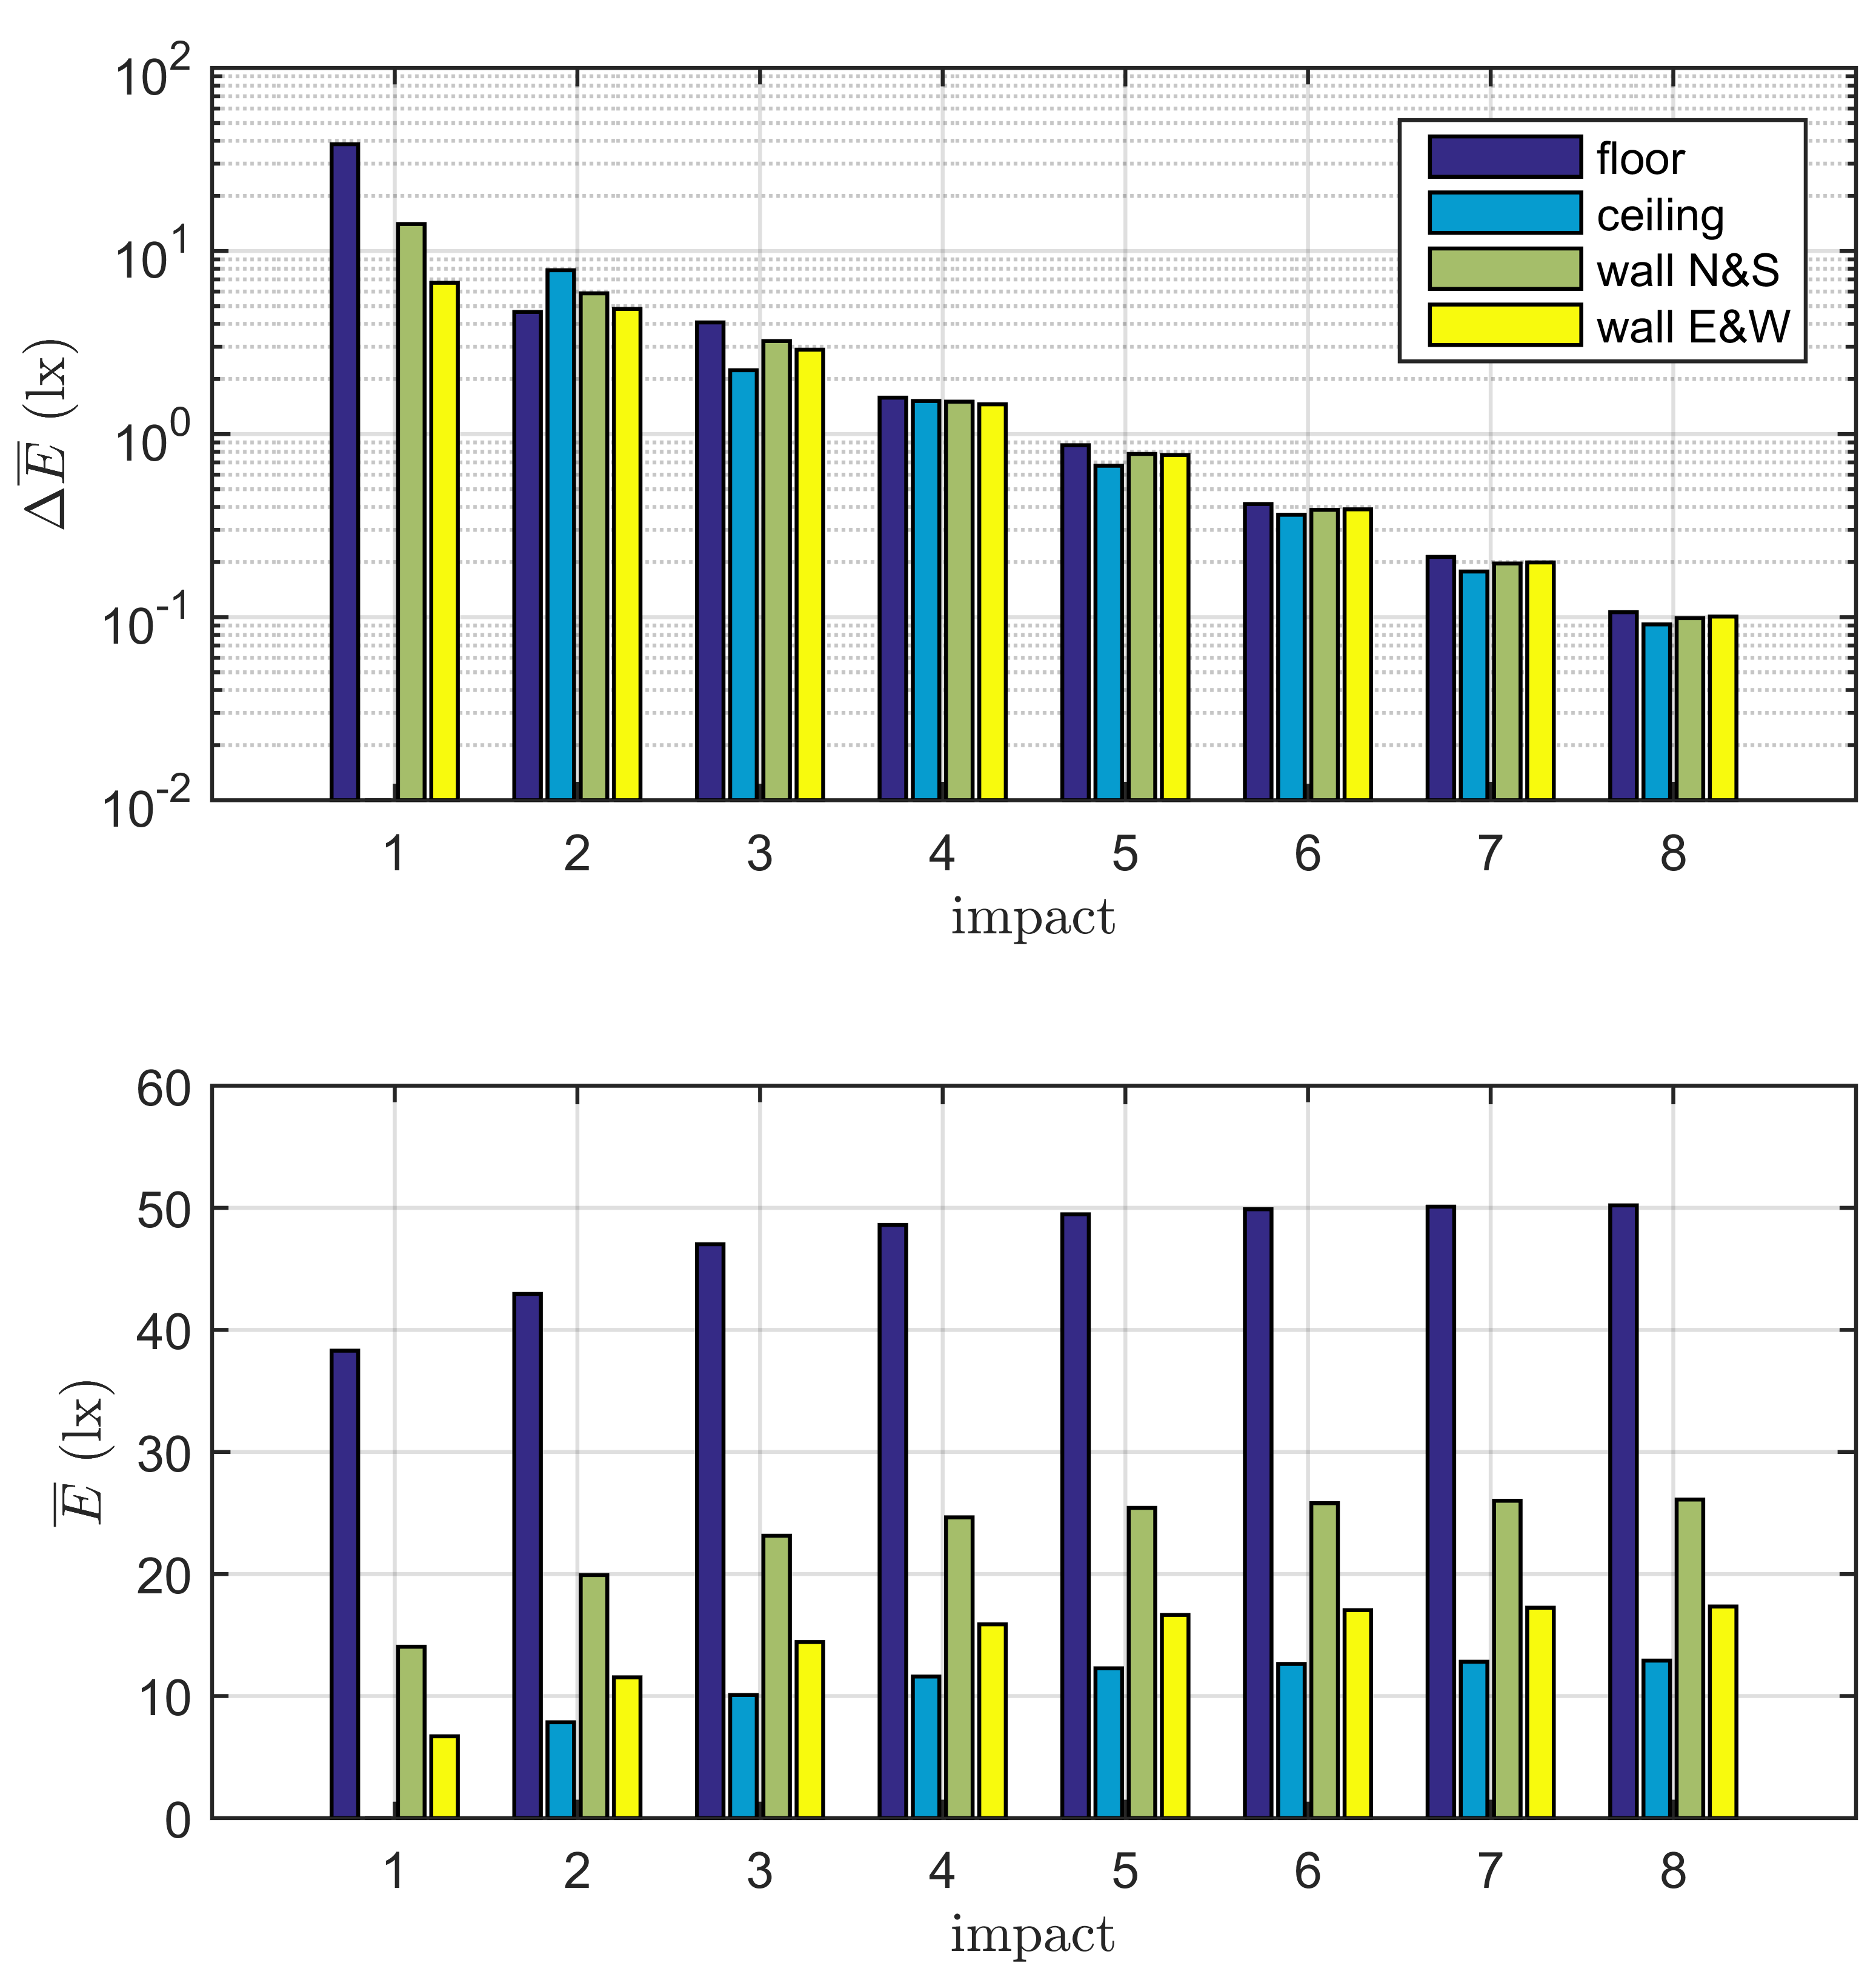
\includegraphics[width=\columnwidth]{reflDif}
  \caption{Increase of the average wall illuminance for one lamp mounted in the center of the room's ceiling depending on the count of reflections.}
  \label{fig:reflDif}
\end{figure}

The grid of evenly spaced control points was placed on the reference plane with distances 25~cm between neighboring points. The luminaires were placed in a rectangular area on the ceiling that starts $0.5$~m from the E\&W walls and $0.4$~m from N\&S walls. All further presented results were evaluated for the same luminaire  MSTR~SLB~4x18W. The luminaire's spacial luminous intensity distribution data were taken from the software "Building Design". All placed luminaires were equally oriented, being described by a normal vector of the $C0^\circ-C180^\circ$ plane in each test. The luminuous intensity curve of the used luminaire is shown in Figure~\ref{fig:IDiag}. The considered dimension of the luminaire were $595\times 595\times 80$~mm.

\begin{figure}[htb]
  \centering
  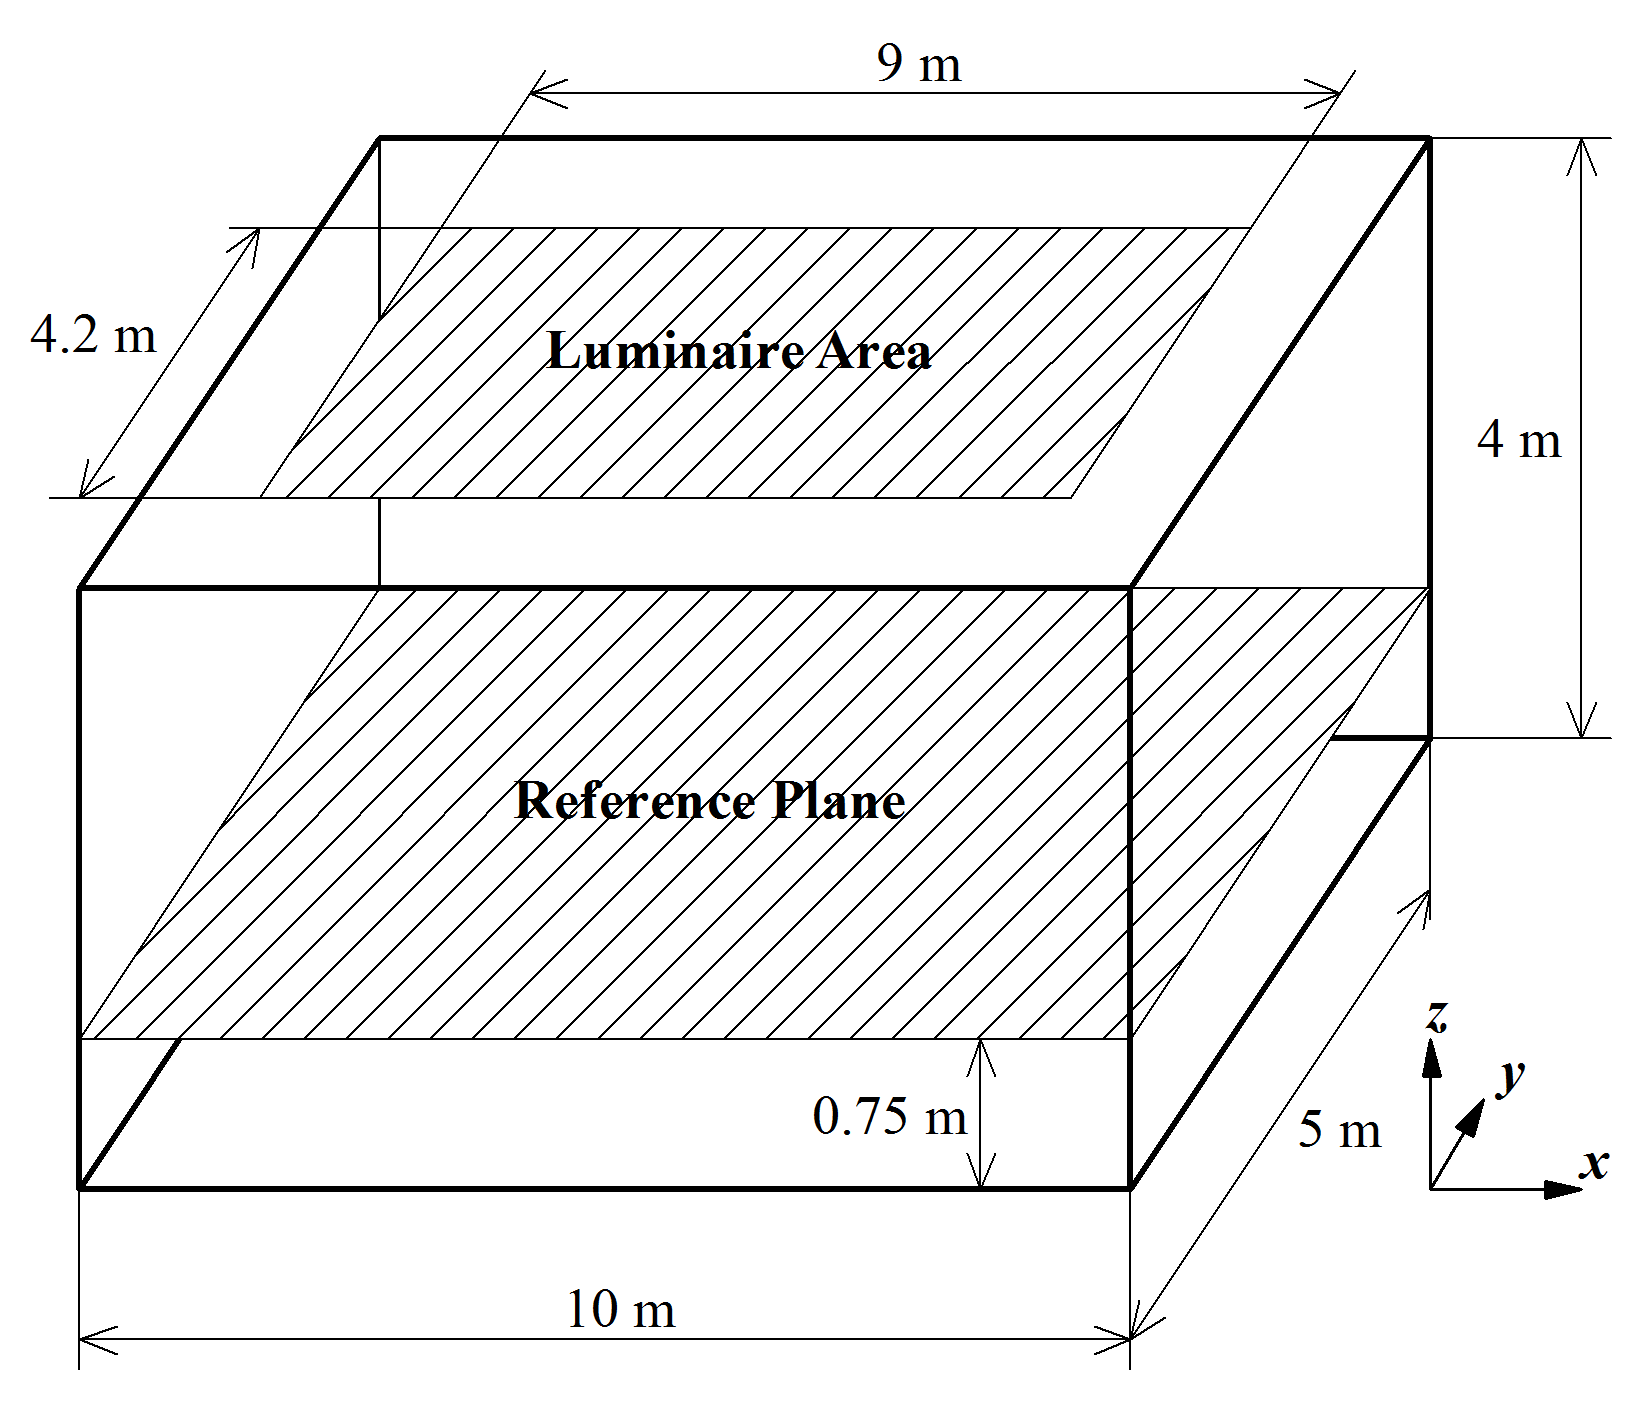
\includegraphics[width=\columnwidth]{modRoom}
  \caption{Model room dimensions}
  \label{fig:modRoom}
\end{figure}

\begin{figure}[htb]
  \centering
  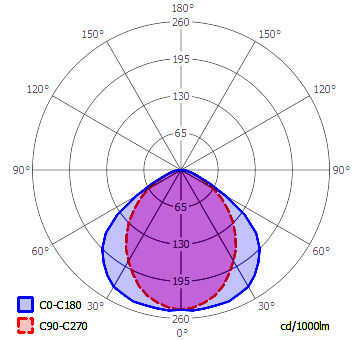
\includegraphics[width=0.8\columnwidth]{IDiag}
  \caption{Luminous intensity distribution curve of the luminaire MSTR SLB 4x18W}
  \label{fig:IDiag}
\end{figure}